%% ------------------------------------------------------------------------- %%
\chapter{Introdução}
\label{cap:introducao}

\section*{Do mundo real ao problema computacional.}
\label{sec:real_computacional}

São Paulo é a segunda maior cidade do mundo em número de restaurantes. Conhecida como a Capital Latino-Americana de boa mesa, possui mais de 15 mil restaurantes, 500 churrascarias, 4.500 pizzarias, 20 mil bares, entre outros \cite{VisiteSaoPaulo}. Dessa forma, encontrar um estabelecimento gastronômico dentre mais de 40 mil opções é uma tarefa impraticável. Surge então a demanda por formas de encontrar uma opção desejada sem métodos exaustivos e de forma eficiente. Para suprir essa demanda, muitas ferramentas de busca atuais utilizam sistemas de Recuperação de Informação (RI).

Segundo Manning, Raghavan e Schütze (2008), Recuperação de Informação é encontrar material (geralmente documentos) de uma natureza não estruturada (geralmente textos) que satisfaça uma informação necessária dentro de grandes coleções (geralmente armazenadas em computadores). Essa área está se tornando rapidamente a forma mais utilizada de acesso a informação, pois permite a recuperação rápida de referências a determinados termos. Isso possibilita aos usuários fazerem buscas de forma não estruturada, utilizando também a linguagem natural. Os resultados são ordenados em alguma ordem de relevância, fazendo emergir resultados que possam ser mais interessantes.

Um dos problemas dessa área é determinar essa ordem em que os resultados devem ser apresentados. Os autores definem a relevância dos resultados como a percepção do usuário sobre as informações contidas no documento e se elas vão de encontro à sua necessidade. Portanto, a relevância é subjetiva ao usuário. Para Crippa e Rodrigues (2011), é justamente essa subjetividade que dificulta alcançar o objetivo da área de fornecer acesso rápido e eficaz às informações relevantes.

A área de RI utiliza estatísticas relacionados a termos e documentos para tentar quantificar essa relevância. Manning, Raghavan e Schütze (2008) dão alguns exemplos de dados que permitem comparar documentos, como a frequência dos termos em um documento, a raridade de um termo na coleção e a quantidade de acessos a uma página Web.

Existem muitos sites na Web que utilizam sistemas de RI, tendo cada um deles formas diferentes de criar consultas e apresentar resultados. Escudeiro e Jorge (2008) definem três abordagens utilizadas por esses sistemas:

\begin{enumerate}
\item \emph{Search-centric approach}: advoga que a busca textual livre se tornou tão boa e seu estilo de interface, tão comum, que os usuários podem satisfazer todas as suas necessidades por meio de consultas simples. Algumas ferramentas de busca utilizam essa abordagem.

\item \emph{Taxonomy navigation approach}: afirma que os usuários têm dificuldades em expressar a informação necessária. Para ajudar a encontrá-la, essa abordagem propõe o uso de estruturas hierárquicas para organizar informações. Um exemplo dessa abordagem são os sistemas de buscas em diretórios.

\item \emph{Meta-data centric approach}: com o auxílio de metadados, podemos filtrar grandes conjuntos de resultados. Algumas ferramentas de busca estão tentando melhorar a qualidade de suas respostas usando evidências diversas, seguindo essa abordagem.

\end{enumerate}

Como exemplo do primeiro modelo, podemos citar o site Google \cite{Google}. Sua busca fornece apenas um campo de texto. Qualquer especificação da busca deve ser feita textualmente. Na sua variante GoogleMaps \cite{GoogleMaps}, o mesmo modelo é utilizado. Nesse site é possível buscar por estabelecimentos como bares e restaurantes. Após a busca ser feita, o usuário tem apenas a opção de filtrar os resultados por uma ``classificação'' que é fornecida pela comunidade.

Este Trabalho de Conclusão de Curso (TCC), por sua vez, se refere ao terceiro modelo, o \emph{meta-data centric approach}. Esse modelo nos orienta a buscar evidências de informações necessárias em outras partes do documento, como o título e os metadados. 

Por exemplo, buscando por sites de restaurantes, um usuário pode achar mais relevantes os resultados com preços mais baixos ou que são mais próximos de sua residência. Pode também querer apenas os restaurantes de melhor qualidade, sem se preocupar com a distância e preço.

Para satisfazer essa necessidade do usuário, não é suficiente olhar para o corpo do documento. Nos metadados, podemos guardar o preço médio das refeições e a coordenada geográfica do estabelecimento. Utilizamos essas informações para filtrar e ranquear os resultados. Nesse modelo, portanto, o usuário tem mais liberdade para comunicar sua necessidade e atuar sobre o ranqueamento dos resultados, contrapondo o primeiro modelo. 

A forma como essa busca é feita varia com a interface que é apresentada para o usuário. Sites como o GuiaFolha \cite{GuiaFolha} e o Kekanto \cite{Kekanto} utilizam um esquema de caixas de seleção para ajudar o usuário a encontrar os resultados mais relevantes. Como podemos ver na figura \ref{fig:interfguiafolha}, existem muitas opções disponíveis que, mesmo agrupadas, podem formar diversas combinações.

%colocar a figura
\begin{figure}[!h]
  \centering
  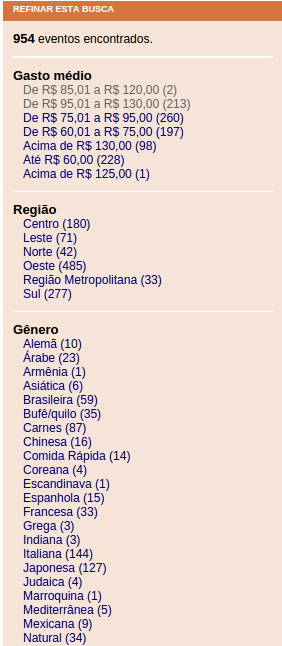
\includegraphics[width=.30\textwidth]{filtroGuiaFolha.png} 
  \caption{Interface do site GuiaFolha \cite{GuiaFolha}}
  \label{fig:interfguiafolha} 
\end{figure}


Por exemplo, é possível filtrar os restaurantes com gasto médio entre R\$75 e R\$95 e que se situam no bairro do Butantã. Não é possível, no entanto, ordenar os resultados por proximidade e preços, balanceando os dois parâmetros de alguma forma. Se o usuário não tem certeza de que filtros usar, precisa testar configurações diferentes, possivelmente realizando várias buscas até encontrar um resultado satisfatório.

Assim, este trabalho tem como principal objetivo desenvolver uma alternativa de busca baseada em metadados de modo a viabilizar a implementação de uma aplicação web que auxilie os usuários a encontrar restaurantes de acordo com alguns poucos critérios, visando simplificar buscas que utilizam metadados.